
\documentclass[11pt,fleqn]{article} 
\usepackage[margin=0.8in, head=0.8in]{geometry} 
\usepackage{amsmath, amssymb, amsthm}
\usepackage{fancyhdr} 
\usepackage{palatino, url, multicol}
\usepackage{graphicx, pgfplots} 
\usepackage[all]{xy}
\usepackage{polynom} 
%\usepackage{pdfsync} %% I don't know why this messes up tabular column widths
\usepackage{enumerate}
\usepackage{framed}
\usepackage{setspace}
\usepackage{array,tikz}

\pgfplotsset{compat=1.6}

\pgfplotsset{soldot/.style={color=black,only marks,mark=*}} \pgfplotsset{holdot/.style={color=black,fill=white,only marks,mark=*}}


\pagestyle{fancy} 
\lfoot{}
\rfoot{\S 2.1}

\begin{document}
\renewcommand{\headrulewidth}{0pt}
\newcommand{\blank}[1]{\rule{#1}{0.75pt}}
\newcommand{\bc}{\begin{center}}
\newcommand{\ec}{\end{center}}
\renewcommand{\d}{\displaystyle}

\vspace*{-0.7in}

%%%%%%%%%intro page
\begin{center}
  \large
  \sc{Section 2.1: Area Between Curves}\\
\end{center}

\begin{enumerate}
\item The graph of the function $\displaystyle g(x) = \frac{e^{\sqrt{x}}}{3\sqrt{x}}$ is graphed below. On the same axes, sketch the graph of $f(x)=6-x$. Then set up an integral or integrals that will calculate the area \emph{between} $f(x)$ and $g(x)$ on the interval from $x=1$ to $x=4.$\\

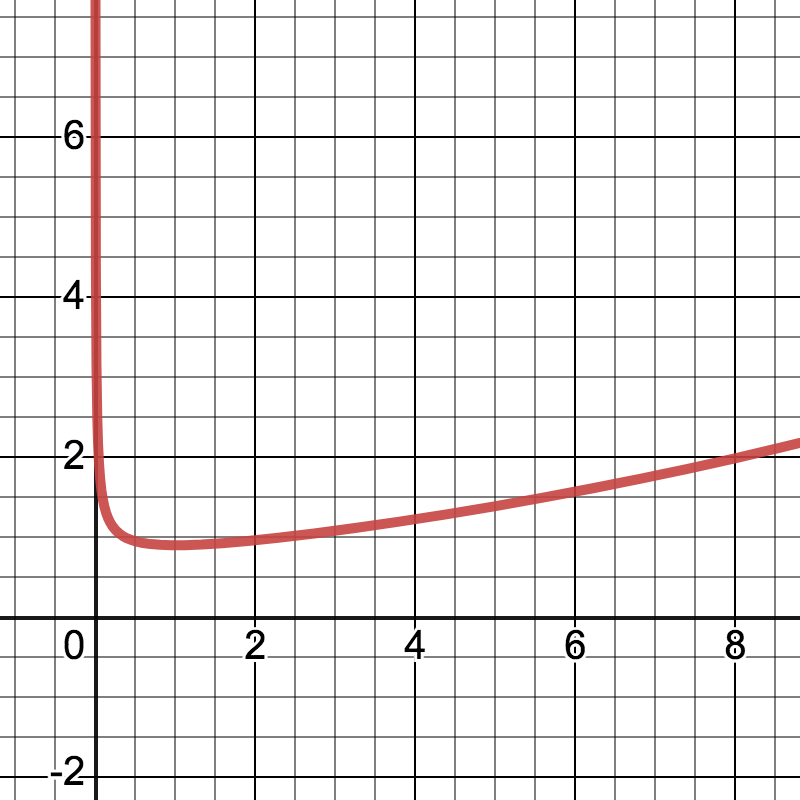
\includegraphics[scale=0.2]{pic-2-1.png}



\item Theorem 2.1: Let $f(x)$ and $g(x)$ be continuous on $[a,b]$ and $f(x) \geq g(x)$ always. Then the area of the region $R$ bounded above by \hspace{1.3cm}, below by \hspace{1.3cm}, on the left by \hspace{1.4cm}, and on the right by  \quad\quad\quad\hspace{1cm}, is given by\\

\vspace{2in}

\item Sketch the region $R$ bounded by $y=4-x^2$ and $y=(x-2)^2.$ Determine the points of intersection and set up an integral to calculate the area of $R.$ Include a sample rectangle in your sketch. Evaluate the integral, if time permits.
\vfill
\newpage
\begin{center} Variations on a Theme \end{center}
\item Sketch the region bounded by $y=x^{1/3},$ $y=1$, $x=-8$ and $x=8.$  Include a sample rectangle in your sketch. Set up an integral to calculate its area.  Evaluate the integral, if time permits.
\vfill
\item Both problems below concern the same region, $R$ (sketched below), bounded on three sides by $y=2$, $y=\frac{1}{x}$, and $y=\frac{x^2}{8}.$\\
	\begin{enumerate}
	\item On the graph below, label each curve with its algebraic formula and the coordinates of each point of intersection. Include sample rectangles in your sketch and use them to set up two integrals to find the area of $R$. 
	
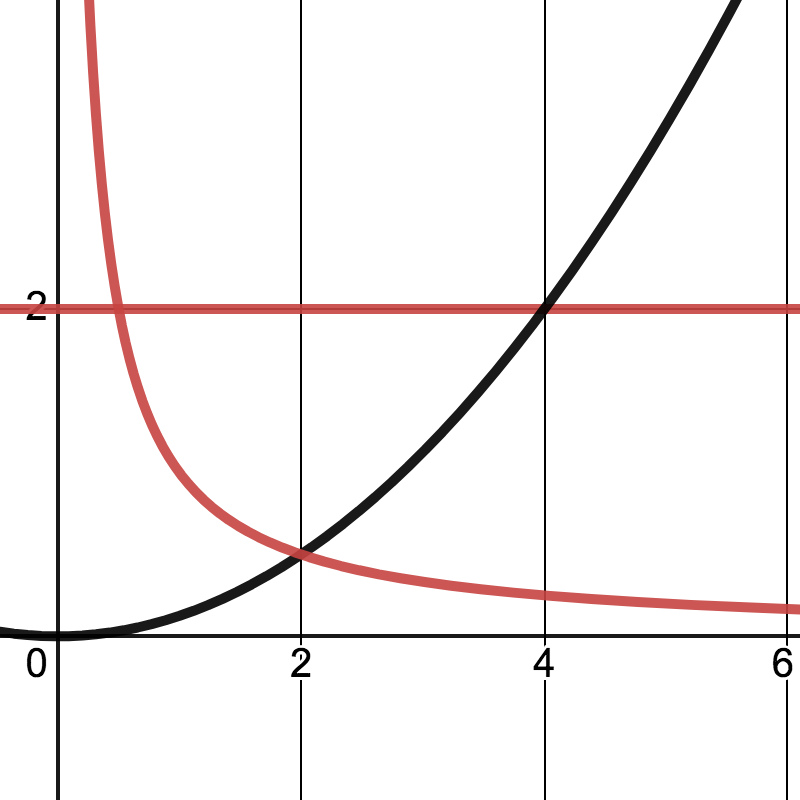
\includegraphics[scale=0.15]{pic-2-1-b.png}
\item On the graph below, label each curve with its algebraic formula \emph{solved for $x$ instead of $y$}, if possible.  Sketch \emph{horizontal} sample rectangles and use them to set up \emph{one} integral that calculates the area of $R$. 
	
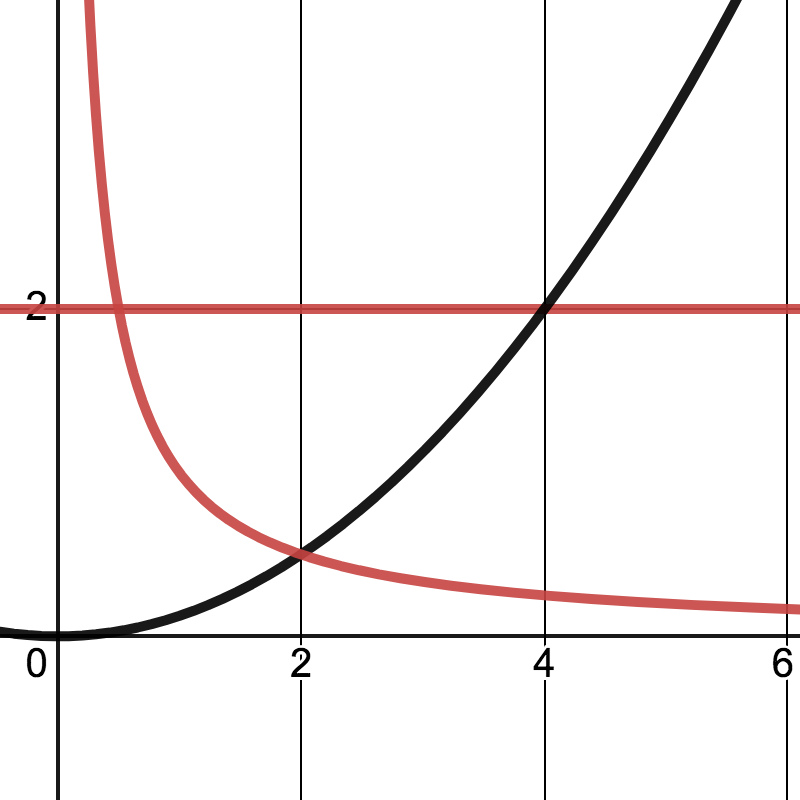
\includegraphics[scale=0.15]{pic-2-1-b.png}
\item What are the pros and cons of using vertical versus horizontal slices?
\end{enumerate}


\end{enumerate}
\end{document}

